\section{Desarrollo}

  \subsection{Consideraciones generales}
    Las imagenes que se utilizan como entrada y salida de los algoritmos a implementar son matrices de píxeles. Cada uno de estos píxeles está representado por cuatro enteros sin signo de 8 bits de profundidad (es decir, en el rango [0, 256)), que contienen, respectivamente, los valores de los colores azul (\textsf{b}), verde (\textsf{g}) y rojo (\textsf{r}), y la transparencia (\textsf{a}).

    Se usará la notación $I_{x,y}$ para referirse al píxel ubicado en la fila $x$ y la columna $y$ de la imagen $I$, y la notación $I_{x,y}^k$ para hacer referencia al valor de la componente $k$ de este píxel, donde $k \in \lbrace \mathsf{b, g, r, a} \rbrace$.
  
  \subsection{Diferencia de imágenes}
    Este filtro recibe dos imágenes como entrada y devuelve como salida una tercera imagen que muestra, en cada píxel, la diferencia entre los píxeles correspondientes de las imágenes de entrada, ignorando la componente \textsf{a}. Más especificamente, si $I_1$ e $I_2$ son las imágenes de entrada y $O$ es la imagen de salida, entonces:

    \[ O_{x,y}^k = \begin{cases}
      \displaystyle \max_{k \in \lbrace \mathsf{b, g, r} \rbrace} \left( \left\vert {I_1}_{x,y}^k - {I_2}_{x,y}^k \right\vert \right)
        & \text{si } k \in \lbrace \mathsf{b, g, r} \rbrace \\
      255
        & \text{si } k = \mathsf{a}
    \end{cases} \]

    \subsubsection{Implementación en lenguaje C}
      La implementación de este filtro en lenguaje C es sumamente sencilla. Ambas imágenes de entrada se recorren simultáneamente mediante dos ciclos anidados, que iteran sobre sus filas y sus columnas, respectivamente. Para las componentes \textsf{b}, \textsf{g} y \textsf{r} de cada píxel, se calcula el valor absoluto de la diferencia entre los valores correspondientes a ambas imágenes. Luego, se computa el máximo entre estos tres valores, que se guarda como el valor de las componentes \textsf{b}, \textsf{g} y \textsf{r} para el píxel correspondiente en la imagen de salida. Por último, la componente \textsf{a} de dicho píxel se define como 255.

    \subsubsection{Implementación en lenguaje ensamblador}
      Al implementar el filtro en lenguaje ensamblador, es posible aprovechar las ventajas que brinda el modelo \acr{SIMD}. En particular, dado que los registros \texttt{XMM} son de 16 bytes, se los puede utilizar para procesar 4 píxeles de las imágenes en paralelo, reduciendo la cantidad de iteraciones del algoritmo y, particularmente, de accesos a memoria necesarios para completar el algoritmo.

      La implementación en este lenguaje del filtro consiste principalmente de un ciclo que itera sobre la imagen. Al comienzo de cada ejecución, se copian 4 píxeles de $I_1$ al registro \texttt{XMM0}, y los correspondientes 4 píxeles de $I_2$ a \texttt{XMM1}.

      \raisebox{2.5mm}{\texttt{XMM0:} } \begin{TAB}(b,1cm,.8cm)[5pt]{|c|c|c|c|c|c|c|}{|c|}
        $A_4^{\mathsf{b}}$ &
        $A_4^{\mathsf{g}}$ &
        $A_4^{\mathsf{r}}$ &
        $A_4^{\mathsf{a}}$ &
        $A_3^{\mathsf{b}}$ &
        $\cdots$ &
        $A_1^{\mathsf{a}}$ \\
      \end{TAB}

      \raisebox{2.5mm}{\texttt{XMM1:} } \begin{TAB}(b,1cm,.8cm)[5pt]{|c|c|c|c|c|c|c|}{|c|}
        $B_4^{\mathsf{b}}$ &
        $B_4^{\mathsf{g}}$ &
        $B_4^{\mathsf{r}}$ &
        $B_4^{\mathsf{a}}$ &
        $B_3^{\mathsf{b}}$ &
        $\cdots$ &
        $B_1^{\mathsf{a}}$ \\
      \end{TAB}

      El paso siguiente consiste en calcular, para cada una de las componentes de estos píxeles, el valor absoluto de la diferencia entre ambas imágenes. Para realizar esto, se realiza la resta de las dos maneras posibles, obtenie $\mathtt{XMM0} = \mathtt{XMM0} - \mathtt{XMM1}$ y $\mathtt{XMM1} = \mathtt{XMM1} - \mathtt{XMM0}$. En las posiciones donde el valor contenido en \texttt{XMM0} sea mayor que el de \texttt{XMM1}, será válido el resultado de la primera operación, mientras que en las demás posiciones se deberá tener en cuenta el segundo resultado.

      Para seleccionar cuál de los dos resultados es el correcto, se utiliza una máscara que se obtiene comparando los valores de \texttt{XMM0} y \texttt{XMM1}. Aquí aparece un problema, ya que debemos comparar enteros sin signo, y \acr{SSE} no brinda instrucciones para hacer esto. Es por eso que se recurre a desempaquetar los números y considerarlos como enteros con signo de dos bytes, que sí se pueden comparar. Empaquetando luego el resultado obtenido, se logra la máscara buscada. Esta se aplica mediante \texttt{PAND} al valor contenido en \texttt{XMM0} y mediante \texttt{PANDN} al valor presente en \texttt{XMM1}. Posteriormente se computa un \texttt{POR} entre los valores recién calculados, llegando al valor deseado, que se almacena en \texttt{XMM0}.

      Por último, es necesario calcular la norma infinito de las componentes \textsf{b}, \textsf{g} y \textsf{r} obtenidas. Para hacer esto, se copia en \texttt{XMM1} el último resultado y se lo desplaza un byte hacia la izquierda.

      \raisebox{2.5mm}{\texttt{XMM0:} } \begin{TAB}(b,1cm,.8cm)[5pt]{|c|c|c|c|c|c|c|c|}{|c|}
        $C_4^{\mathsf{b}}$ &
        $C_4^{\mathsf{g}}$ &
        $C_4^{\mathsf{r}}$ &
        $C_4^{\mathsf{a}}$ &
        $C_3^{\mathsf{b}}$ &
        $C_3^{\mathsf{g}}$ &
        $\cdots$ &
        $C_1^{\mathsf{a}}$ \\
      \end{TAB}

      \raisebox{2.5mm}{\texttt{XMM1:} } \begin{TAB}(b,1cm,.8cm)[5pt]{|c|c|c|c|c|c|c|c|}{|c|}
        0 &
        $C_4^{\mathsf{b}}$ &
        $C_4^{\mathsf{g}}$ &
        $C_4^{\mathsf{r}}$ &
        $C_4^{\mathsf{a}}$ &
        $C_3^{\mathsf{b}}$ &
        $\cdots$ &
        $C_1^{\mathsf{a}}$ \\
      \end{TAB}

      A continuación puede usarse la instrucción \texttt{PMAXUB XMM1, XMM0} para calcular el máximo entre estos dos registros, obteniendo 

      \raisebox{2.5mm}{\texttt{XMM1:} } \begin{TAB}(r,1cm,.8cm)[5pt]{|c|c|c|c|c|c|c|c|c|}{|c|}
        \makebox[.8cm]{\texttt{*}} &
        $\max(C_4^{\mathsf{b}}, C_4^{\mathsf{g}})$ &
        \makebox[.8cm]{\texttt{*}} &
        \makebox[.8cm]{\texttt{*}} &
        \makebox[.8cm]{\texttt{$\cdots$}} &
        \makebox[.8cm]{\texttt{*}} &
        $\max(C_1^{\mathsf{b}}, C_1^{\mathsf{g}})$ &
        \makebox[.8cm]{\texttt{*}} &
        \makebox[.8cm]{\texttt{*}}  \\
      \end{TAB}

      Repitiendo el proceso anterior, pero esta vez almacenando el resultado en \texttt{XMM0}, se obtiene

      \raisebox{2.5mm}{\texttt{XMM0:} } \begin{TAB}(r,1cm,.8cm)[5pt]{|c|c|c|c|c|c|c|c|c|}{|c|}
        \makebox[.7cm]{\texttt{*}} &
        \makebox[.7cm]{\texttt{*}} &
        $\max(C_4^{\mathsf{b}}, C_4^{\mathsf{g}}, C_4^{\mathsf{r}})$ &
        \makebox[.7cm]{\texttt{*}} &
        \makebox[.7cm]{\texttt{$\cdots$}} &
        \makebox[.7cm]{\texttt{*}} &
        \makebox[.7cm]{\texttt{*}} &
        $\max(C_4^{\mathsf{b}}, C_4^{\mathsf{g}}, C_4^{\mathsf{r}})$ &
        \makebox[.7cm]{\texttt{*}}  \\
      \end{TAB}

      A partir de aquí, utilizando la instrucción \texttt{PSHUFB} para replicar el valor calculado, se almacena este máximo en las componentes \textsf{r}, \textsf{g} y \textsf{b} de los píxeles correspondientes de la imagen de destino, y utilizando una máscara adecuada, se define la componente \textsf{a} de todos ellos como 255.

  \subsection{Blur gaussiano}
    Este filtro recibe una imagen como entrada y devuelve como salida el resultado de aplicarle una convolución\footnote{Dadas dos funciones $f$ y $g$, una \emph{convolución} $f * g$ es una operación que las transforma en una tercera función: $(f * g)(t) = \int_{-\infty}^{+\infty} f(\tau) g(t - \tau) \,d\tau$ en el caso continuo, $(f * g)_n = \sum_{k=-\infty}^{+\infty} f_k g_{n-k}$ ($n, k \in \mathbb{Z}$) en el caso discreto.} con una función gaussiana, que dependerá de un parámetro $\sigma$ que podrá ser modificado. Dada la naturaleza del problema, trabajaremos con una convolución discreta en dos dimensiones, y como nuestro poder de cómputo es limitado, procesaremos solo una vecindad acotada de cada píxel, cuyo radio quedará determinado por un parámetro configurable $r$. En definitiva, el resultado del filtro será

    \[ O_{x,y}^k = \begin{cases}
      \displaystyle \sum_{i=-r}^r \sum_{j=-r}^r O_{x+i,y+j}^k K_{r-i,r-j}
        & \text{si } k \in \lbrace \mathsf{b, g, r} \rbrace \\
      255
        & \text{si } k = \mathsf{a}
    \end{cases} \]

    donde $K$ es la matriz o \emph{kernel} de la convolución, con

    \[ K_{i,j} = \frac{1}{2 \pi \sigma^2} e^{- \frac{(r-i)^2 + (r-j)^2}{2 \sigma^2}} \qquad \text{para todo } 0 \leq i,j \leq 2r \]

    \subsubsection{Implementación en lenguaje C}

      Para aplicar el filtro, es necesario que el parámetro $r$ sea menor que la mitad de la cantidad de filas y menor que la mitad de la cantidad de columnas. Por esto, verificamos que el parámetro cumpla con estas condiciones. El siguiente paso consiste en crear la matriz de convolución del filtro llamando a una función auxiliar, explicada más adelante. 

      Luego, mediante dos ciclos, se recorre toda la parte de la imagen original a la que es posible aplicarle el filtro. Esta parte es la que contempla las filas desde el valor del radio hasta $filas - (r + 1$), y las columnas desde el valor del radio hasta $columnas - (r + 1$). El resto de la imagen no será afectada. 

        {\centering \begin{tabular}{c}
          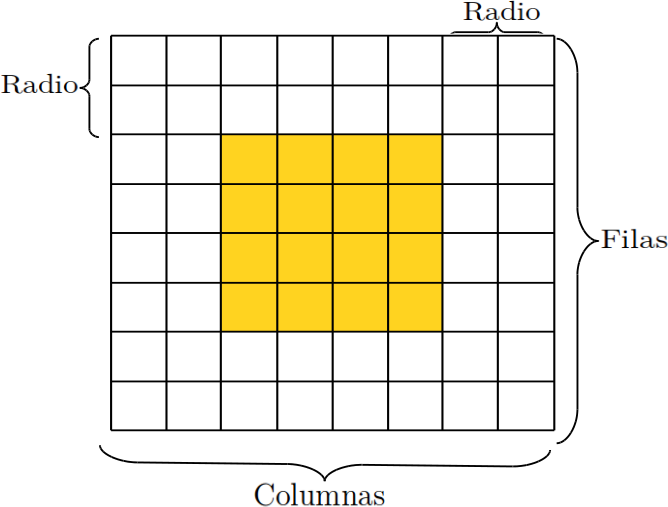
\includegraphics[width=7cm]{./imagenes/1.png} \\
        \end{tabular}}

      En cada paso de esta iteración, se llama a la función \texttt{afectarPixel}, que se ocupa de modificar cada píxel correctamente, utilizando la matriz de convolución creada anteriormente. 

      \subsubsection*{Función \texttt{matrizDeConvolucion}}

        En esta parte del algoritmo se calcula la matriz de la convolución. Para ello, en primer lugar, se piden $4 \times (2r + 1)^2$ bytes de memoria, lugar que va a ocupar la matriz ya que su altura es $2r + 1$ y su ancho, $4 \times (2r 1)$ (porque cada píxel ocupa 4 bytes).
        
        Se utilizan dos ciclos; ambos van desde 0 hasta $2r + 1$. 
        
        {\centering \begin{tabular}{c}
          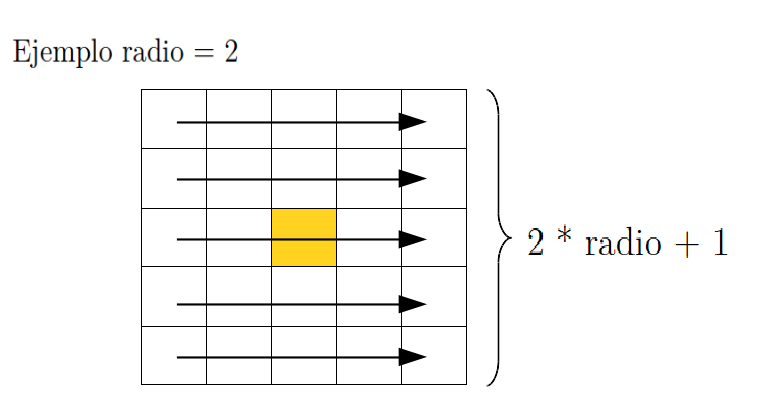
\includegraphics[width=7cm]{./imagenes/2.png} \\
        \end{tabular}}

        En cada paso, se calcula la función gaussiana con el $\sigma$, $r$, $i$ y $j$ correspondientes, donde $i$ representa la fila y $j$ la columna. Luego, se coloca el resultado en la fila $i$, columna $j$ de la matriz. Finalmente, se devuelve un puntero a la primera posición de la matriz.

      \subsubsection*{Función \texttt{afectarPixel}}
        Primero se inicializan 3 variables donde luego se van a almacenar las sumas que corresponden a cada componente del píxel a afectar (\textsf{b}, \textsf{g} y \textsf{r}). 

        Seguidamente, se utilizan dos ciclos para recorrer la matriz de convolución y la parte de la imagen correspondiente a los vecinos del píxel a afectar. 
        
        Estos van desde $0$ hasta $(2r)$, para recorrer las filas, y desde $0$ hasta $(2r \times 4)$ para recorrer las columnas. En cada paso se multiplica el valor de las componentes del píxel observado por el valor de la matriz de convolución. El resultado de esta multiplicación se suma en las 3 variables creadas en el principio. 
        
        Finalmente, se copia el valor de cada variable en cada componente del píxel en la imagen destino. Luego, en la componente \textsf{a} se coloca el valor 255.  

    \subsubsection{Implementación en lenguaje ensamblador} 
      Este algoritmo se ocupa de recorrer toda la porción de la imagen a la que es posible aplicarle el filtro. 
      
      Al igual que en la implementación en C, primero se hace una comparación para revisar si el radio es válido. 
      
      Luego, utilizando la instrucción \texttt{CALL}, se hace un llamado a la función \texttt{matrizDeConvolución} (implementada en C), la cual devuelve un puntero a la matriz de convolución creada. 
      
      Posteriormente, se utilizan dos ciclos para recorrer la porción a modificar de la imagen. Estos utilizan los registros \texttt{R8} para recorrer las columnas y \texttt{R9} para recorrer las filas.

        {\centering \begin{tabular}{c}
          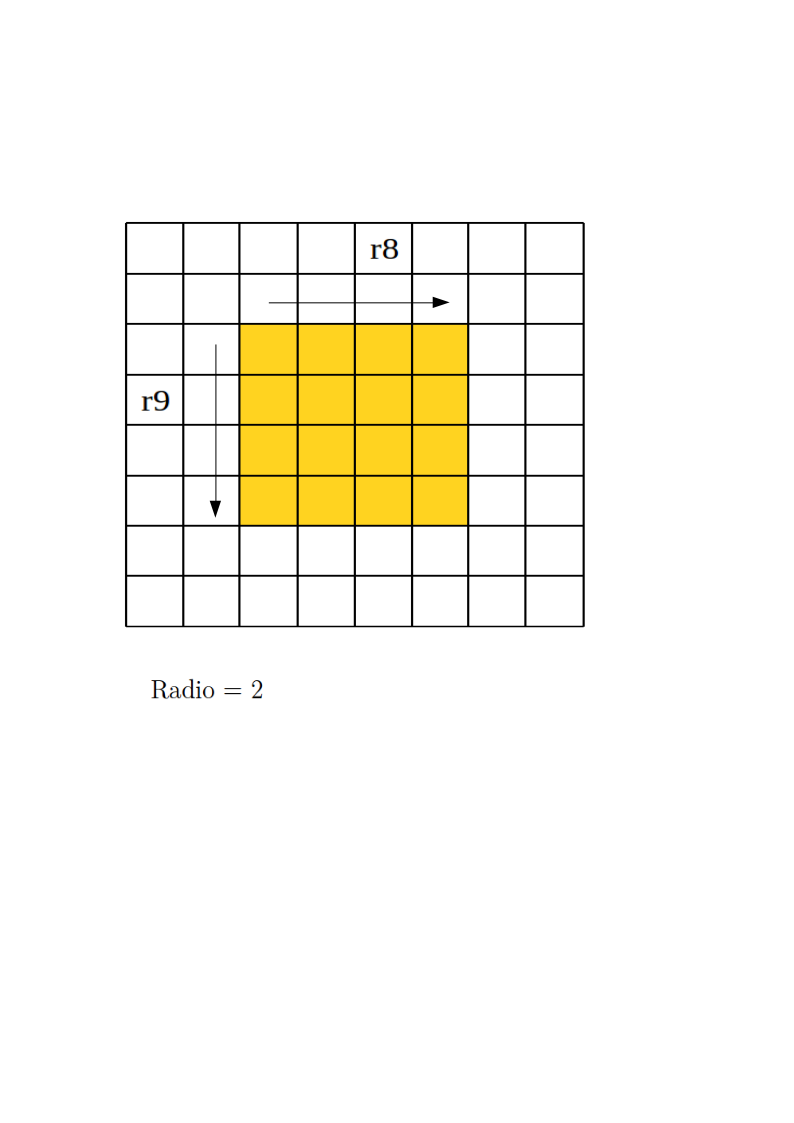
\includegraphics[width=7cm]{./imagenes/4bis.png} \\
        \end{tabular}}

      En cada paso del ciclo, utilizando nuevamente la instrucción \texttt{CALL}, se realiza un llamado a la función afectarPixel (implementada en assembler) que se ocupa de modificar el píxel correspondiente. 

      \paragraph{Función \texttt{afectarPixel}}
        El primer paso de este algoritmo es encontrar el puntero al píxel que se debe afectar en la imagen original y otro puntero al mismo píxel pero en la imagen destino. Estos punteros son guardados en los registros \texttt{R12} y \texttt{R14}, respectivamente.   

        Llamaremos \emph{submatriz imagen} a la porción de la imagen original que se debe utilizar para que, junto con la matriz de convolución, se obtenga el nuevo valor del píxel. Esta submatriz es la que contiene al píxel a modificar en el centro y su tamaño es el mismo que el de la matriz de convolución. 
        
        {\centering \begin{tabular}{c}
          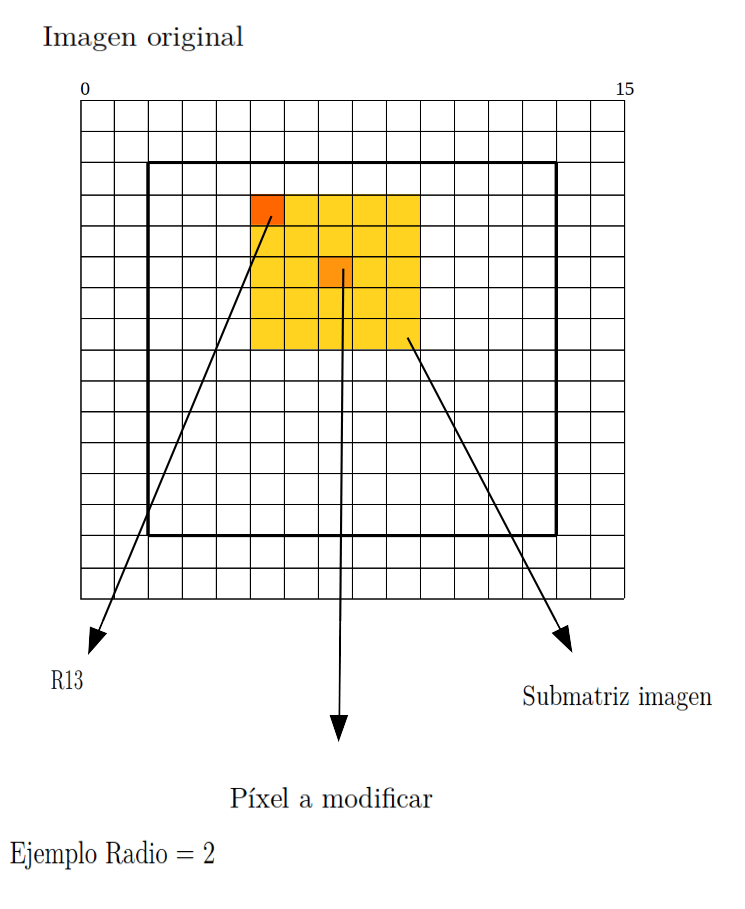
\includegraphics[width=7cm]{./imagenes/5.png} \\
        \end{tabular}}

        Luego, se debe encontrar el puntero al primer píxel de la submatriz imagen. Esto se calcula de la siguiente manera: $\mathtt{R12} - 4 \times (r - r \times columnas)$. Este puntero se encuentra en el registro r13 y es utilizado para recorrer la submatriz. 

        En el registro \texttt{R11} se guarda la cantidad total de píxeles que componen la submatriz imagen. 

              $\mathtt{R11} = (2 \times r + 1)^{2}$  
        
        El registro \texttt{R15} contiene el tamaño de las filas.
        
              $\mathtt{R15} = (2 \times r + 1)$

        Estos últimos dos se utilizan como registros contadores.

        A continuación, se recorren por filas la submatriz imagen y la matriz de convolución a la vez. \texttt{R11} se utiliza para saber cuando finalizar el bucle, es decir, cuando ya se observaron todos los píxeles. Estos son procesados utilizando instrucciones \acr{SSE} y registros del tipo \texttt{XMM}. En cada uno de estos registros es posible guardar 4 píxeles, ya que cada píxel ocupa 4 bytes. 

        {\centering \begin{tabular}{c}
          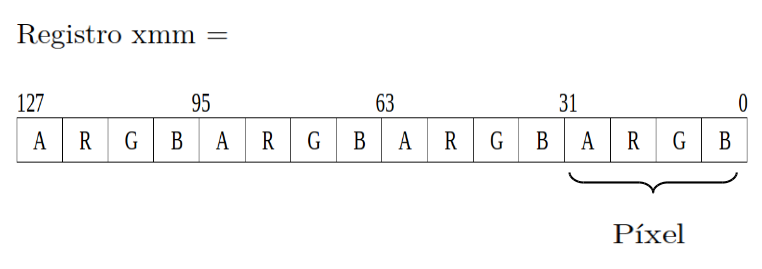
\includegraphics[width=7cm]{./imagenes/6.png} \\
        \end{tabular}}
  
        En cada paso de este ciclo se considera una fila, utilizando \texttt{R15} para saber cuándo termina. Se toman 4 píxeles de la submatriz imagen y los correspondientes 4 de la matriz de convolución. Luego de desempaquetar los píxeles se realiza la multiplicación de cada componente (\textsf{b}, \textsf{g} o \textsf{r}) con el valor de la matriz de convolución que le corresponde. El resultado de cada producto se suma al registro \texttt{XMM6}. 

        {\centering \begin{tabular}{c}
          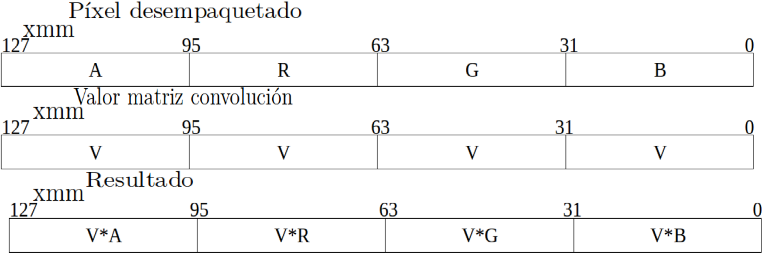
\includegraphics[width=7cm]{./imagenes/3bis.png} \\
        \end{tabular}}

        Se puede notar que el tamaño de las filas es congruente a 1 o 3 módulo 4. 
        CUENTA1. Por lo tanto, se procesan de a 4 píxeles hasta llegar a alguno de los dos casos borde posibles: cuando queda 1 píxel por computar o cuando quedan 3. 
        
        La solución a este problema es tomar y desempaquetar los píxeles de la submatriz imagen que todavía no fueron procesados junto con sus siguientes, hasta completar 4. Esto es así en todos los casos, excepto en el que los píxeles restantes son los últimos de la submatriz imagen (es decir, los que se corresponden con la última fila). En este caso, se toman los píxeles anteriores, ya que de otra forma, si el píxel a modificar se encontrase en alguna de las 3 últimas posiciones se accedería a posiciones de memoria fuera de la imagen. Estos píxeles no se tienen en cuenta a la hora de realizar el cálculo.

        Esto mismo se realiza para la matriz de convolución.
          
        {\centering \begin{tabular}{cc}
          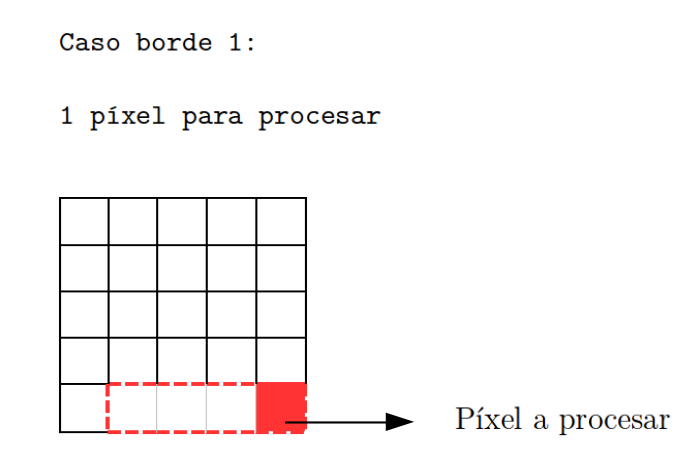
\includegraphics[width=7cm]{./imagenes/7.png} &
          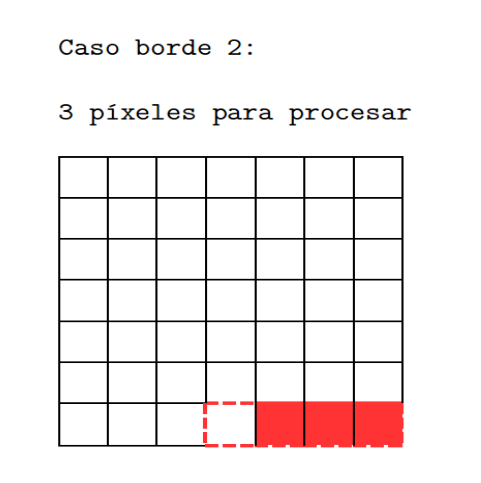
\includegraphics[width=7cm]{./imagenes/8.png}
          \\
        \end{tabular}}

        Al finalizar el ciclo, se tiene en \texttt{XMM6} el valor esperado para cada componente (\textsf{b}, \textsf{g} y \textsf{r}) del píxel a afectar, en punto flotante de 32 bits. Primero se pasan estos valores a enteros; después, en la componente \textsf{a} se coloca un 255, y luego se empaqueta \texttt{XMM6} para copiarlo en la posición del píxel que se quiere modificar en la imagen destino.
